\documentclass[11pt,a4paper]{ctexart}
\usepackage[teacher]{ipara}

\pagestyle{fancy}
\fancyhf{}
\lhead{\small 公共专题教案：函数性态分析总结}
\rhead{\small 教师备课版}
\cfoot{\small 第 \thepage\ 页\quad 共 \zpageref{LastPage} 页}
\renewcommand{\headrulewidth}{0.4pt}
\renewcommand{\footrulewidth}{0pt}

% 自定义双栏排版块标记
\newcommand{\topicteachblock}[2]{%
  \par\addvspace{0.55em}%
  \noindent\textbf{【#1】}\par\nobreak
  \begingroup
    \setlength{\parskip}{0.35em}%
    #2\par
  \endgroup
}

\begin{document}

\begin{center}
  {\LARGE\bfseries 一轮复习专题：函数性态分析 \quad (教师版)}\par
  \vspace{0.8em}
  {\small 建议授课时长：120 分钟 \quad 核心考点：单调性、奇偶性、对称性、周期性}
\end{center}
\vspace{0.6em}

\section{备课指导与时间分配建议}

\begin{teachbox}{本专题教学定位}
  本专题是高考一轮复习中函数模块的灵魂与难点所在。高考对函数性质的考察已由“单一性质的简单套用”转向“多种性质的综合嵌套与抽象推导”（如轴对称与中心对称叠加推周期、单调性与奇偶性复合解不等式）。\\
  在授课过程中，教师必须摒弃“只讲公式、不看前提”的机械记忆法，重点落实以下两点：
  \begin{enumerate}
    \item \textbf{前提意识（定义域优先）}：所有性质的讨论必须在定义域内进行，奇偶性、对称性、周期性的第一步一定是检验定义域的对称性或平移不变性。
    \item \textbf{反例教学（错因精准识别）}：引导学生在理解性质成立的充分条件的同时，牢记经典的“不一定成立”的反例。通过反例剖析逻辑漏洞，形成深刻的条件边界意识。
  \end{enumerate}
\end{teachbox}

\subsection*{课堂 120 分钟时间分配表}
\begin{tabularx}{\textwidth}{p{2.2cm}p{3.0cm}X}
\toprule
时间段 & 教学环节 & 核心动作与重难点点拨\\
\midrule
0--20 分钟 & 板块一：定义域与值域 & 强调定义域是函数的灵魂。剖析偶函数区间不对称、奇函数在零点无定义等经典反例陷阱。\\ \hline
20--50 分钟 & 板块二：单调性深剖 & 讲解增减函数四则运算及倒数运算的“不确定性”，重点剖析反例（如两正增函数乘积才递增、分段单调不等于全局单调）。\\ \hline
50--80 分钟 & 板块三：奇偶性及复合 & 总结复合函数奇偶性“内偶则偶，内奇跟外”的规律，以及奇偶性与单调性在对称区间上的同向/反向特征。\\ \hline
80--115 分钟 & 板块四：对称性与周期 & 利用 TikZ 图形直观展示“两轴推周期”、“两点推周期”、“一轴一点推周期”的代数平移与反射原理，扫除公式死角。\\ \hline
115--120 分钟 & 总结与课后补救 & 提炼核心口诀，布置本讲核心反例的记忆与重写任务。\\
\bottomrule
\end{tabularx}

\newpage

\section{板块一：定义域与值域——一切性质的基石}

\begin{theorembox}{核心原则：定义域优先}
  任何函数的性质（单调性、奇偶性、对称性、周期性）都是在特定定义域下表现出来的。脱离定义域谈函数性质是解析几何与代数中最常见的逻辑错误。
\end{theorembox}

\begin{paracol}{2}
\topicteachblock{基础概念梳理}{
  1. \textbf{定义域的求法}：主要考虑偶次根式被开方数非负、分母不为零、对数真数大于零且底数大于零且不为1、三角函数自变量范围等限制条件。\\
  2. \textbf{奇偶性对称前提}：若函数 $f(x)$ 具有奇偶性，其定义域 $D$ 必须关于原点对称，即对任意 $x \in D$，必有 $-x \in D$。\\
  3. \textbf{值域的依赖性}：值域是自变量在定义域内连续变化时函数值的集合。公式一致但定义域不同，值域与单调性会发生本质改变。
}

\switchcolumn
\topicteachblock{典型学情诊断}{
  学生最容易将“代数式本身的性质”误认为是“函数的性质”，忽略定义域的限制作用。
}
\end{paracol}

\begin{warnbox}{易错警示与经典反例（必须引导学生熟记）}
  \errortag{忽略定义域对称前提}
  \textbf{命题}：若对定义域内任意 $x$，都有 $f(-x) = f(x)$，则 $f(x)$ 必为偶函数。\\
  \textbf{反例}：设函数 $f(x) = x^2$，$x \in [0, +\infty)$。\\
  虽然其代数式满足 $f(-x) = f(x)$ 的形式，但因其定义域 $[0, +\infty)$ 不关于原点对称，故该函数\textbf{既不是奇函数也不是偶函数}。
  \vspace{0.4em}
  \hrule
  \vspace{0.4em}
  \errortag{奇函数零点必过原点陷阱}
  \textbf{命题}：若 $f(x)$ 是奇函数，则必有 $f(0) = 0$。\\
  \textbf{反例}：设函数 $f(x) = \frac{1}{x}$。\\
  该函数在整个定义域 $\mathbb{R} \setminus \{0\}$ 上满足 $f(-x) = -f(x)$，是一个标准的奇函数。然而，由于 $x = 0$ 不在定义域内，$f(0)$ 根本无定义，更无法得出 $f(0)=0$ 的结论。\\
  \textbf{正确定理}：若 $f(x)$ 是奇函数\textbf{且在 $x = 0$ 处有定义}，则必有 $f(0) = 0$。
\end{warnbox}

\newpage

\section{板块二：单调性——增减趋势与运算法则}

\begin{theorembox}{单调性的代数与导数定义}
  设函数 $f(x)$ 在区间 $I$ 上有定义，对任意 $x_1, x_2 \in I$，且 $x_1 < x_2$：
  \begin{itemize}
    \item 若 $f(x_1) < f(x_2)$，则 $f(x)$ 在 $I$ 上单调递增；若 $f(x_1) > f(x_2)$，则 $f(x)$ 在 $I$ 上单调递减。
    \item 若 $f(x)$ 在区间 $I$ 上可导，则 $f'(x) > 0 \implies f(x)$ 单调递增；$f'(x) < 0 \implies f(x)$ 单调递减。
  \end{itemize}
\end{theorembox}

\begin{paracol}{2}
\topicteachblock{复合函数单调性口诀}{
  对于复合函数 $y = f(g(x))$，其单调性遵循\textbf{“同增异减”}法则：
  \begin{itemize}
    \item 外层 $f(u)$ 与内层 $g(x)$ 单调性相同时，复合函数单调递增；
    \item 外层 $f(u)$ 与内层 $g(x)$ 单调性相反时，复合函数单调递减。
  \end{itemize}
  \textbf{极其重要的一点}：在使用复合函数单调性法则前，必须确保内层函数 $g(x)$ 的值域落在外层函数 $f(u)$ 的定义域及对应的单调区间内。
}

\topicteachblock{四则运算单调性规律}{
  \begin{itemize}
    \item \textbf{加法}：增 + 增 = 增；减 + 减 = 减.
    \item \textbf{减法}：增 - 减 = 增；减 - 增 = 减.
    \item \textbf{乘法/除法/倒数}：单调性不具有普适的代数运算法则，必须结合函数正负号或导数符号具体分析。
  \end{itemize}
}

\switchcolumn
\topicteachblock{复合单调性定义域陷阱诊断}{
  学生常直接用“同增异减”做题，完全不检验外层函数的定义域，导致得出不存在的区间。
}
\end{paracol}

\begin{warnbox}{复合单调性失效反例}
  \textbf{反例}：求 $y = \ln(x^2 - 2x)$ 在区间 $[0, 1]$ 上的单调性。\\
  若盲目套用：内层 $g(x) = x^2 - 2x$ 在 $[0, 1]$ 上单调递减，外层 $f(u) = \ln u$ 单调递增，故整体在 $[0, 1]$ 上单调递减。\\
  \textbf{事实上}：当 $x \in [0, 1]$ 时，$x^2 - 2x \le 0$，此时真数位置的 $u \le 0$，外层对数函数\textbf{完全无意义}。该函数的定义域为 $(-\infty, 0) \cup (2, +\infty)$，因此在 $[0, 1]$ 上无定义，根本谈不上单调性。
\end{warnbox}

\begin{warnbox}{四则运算与倒数单调性经典反例（强记）}
  \errortag{单增乘积单增假命题}
  \textbf{命题}：若 $f(x)$ 和 $g(x)$ 在区间 $I$ 上均单调递增，则它们的乘积 $f(x)g(x)$ 在 $I$ 上也单调递增。\\
  \textbf{反例}：设 $f(x) = x$，$g(x) = x$，定义在 $\mathbb{R}$ 上，它们显然在 $\mathbb{R}$ 上单调递增。\\
  然而它们的乘积为 $f(x)g(x) = x^2$。该函数在 $(-\infty, 0)$ 上单调递减，在 $[0, +\infty)$ 上单调递增，反而不是在整个 $\mathbb{R}$ 上单调递增。\\
  \textbf{修正结论}：必须增加条件“$f(x) \ge 0, g(x) \ge 0$”时，增 $\times$ 增 = 增 才能成立。
  \vspace{0.4em}
  \hrule
  \vspace{0.4em}
  \errortag{单增倒数单减假命题}
  \textbf{命题}：若 $f(x)$ 在定义域内单调递增，则其倒数 $\frac{1}{f(x)}$ 在定义域内单调递减。\\
  \textbf{反例}：设函数 $f(x) = x$，$x \in \mathbb{R} \setminus \{0\}$。它在定义域内是递增的。\\
  但其倒数 $g(x) = \frac{1}{x}$ 在整个定义域上并不是单调递减的。例如，取 $x_1 = -1 < x_2 = 1$，则 $g(-1) = -1 < g(1) = 1$，函数值反而变大了，不满足单调递减的定义。\\
  \textbf{修正结论}：只有在 $f(x)$ \textbf{保持恒正或恒负}的连续区间上，递增函数的倒数才是单调递减的。
\end{warnbox}

\newpage

\section{板块三：奇偶性——原点对称与复合运算}

\begin{theorembox}{奇偶性的代数运算与单调性特征}
  \begin{enumerate}
    \item \textbf{四则运算奇偶性（同性相乘除得偶，异性相乘除得奇）}：
          偶 $\times$ 偶 = 偶，奇 $\times$ 奇 = 偶，奇 $\times$ 偶 = 奇（除法同理）。
    \item \textbf{复合函数奇偶性（内偶则偶，内奇跟外）}：
          对于 $F(x) = f(g(x))$，若内层 $g(x)$ 是偶函数，则 $F(x)$ 必为偶函数；若内层 $g(x)$ 是奇函数，则 $F(x)$ 的奇偶性与外层函数 $f(u)$ 的奇偶性一致。
    \item \textbf{奇偶性与单调性的对称关联}：
          \begin{itemize}
            \item \textbf{奇函数}：在关于原点对称的区间上具有\textbf{相同}的单调性；
            \item \textbf{偶函数}：在关于原点对称的区间上具有\textbf{相反}的单调性。
          \end{itemize}
  \end{enumerate}
\end{theorembox}

\begin{paracol}{2}
\topicteachblock{性质应用点拨}{
  在解决抽象不等式时，奇偶性与单调性的结合是最高效的降维工具。
  例如利用偶函数 $f(x) = f(|x|)$ 将负数自变量直接转化为正数，或者利用奇函数 $f(-x) = -f(x)$ 将负号提到外面，再配合单调性去掉抽象符号 $f$，将问题转化为常规代数不等式。
}

\switchcolumn
\topicteachblock{单调区间拼凑陷阱}{
  学生最容易犯的错误是把“各区间单调性相同”等同于“在整个并集区间上单调”。
}
\end{paracol}

\begin{warnbox}{分段单调不等于全局单调反例}
  \errortag{割裂区间的单调性拼凑}
  \textbf{反例}：奇函数 $f(x) = \frac{1}{x}$。\\
  它在 $(-\infty, 0)$ 上是单调递减的，在 $(0, +\infty)$ 上也是单调递减的。\\
  若学生因为“奇函数对称区间单调性相同”而得出结论：“$f(x) = \frac{1}{x}$ 在定义域 $\mathbb{R} \setminus \{0\}$ 上单调递减”，这是完全错误的。\\
  因为取 $x_1 = -1 \in (-\infty, 0)$，$x_2 = 1 \in (0, +\infty)$，虽然 $x_1 < x_2$，但 $f(-1) = -1 < f(1) = 1$，并不满足整个自变量集合上的递减定义。\\
  \textbf{板书规范}：书写单调区间时，若存在断开的区间，\textbf{必须用“和”或逗号连接}，严禁使用并集符号“$\cup$”。
\end{warnbox}

\newpage

\section{板块四：对称性与周期性——代数互推与直观图像}

本板块是函数性质综合题的核心，教师在上课时应着重进行代数公式与图像对称变换的对齐讲解。

\subsection{轴对称与中心对称的代数特征}

\begin{theorembox}{基本对称表达式的识别与互推}
  \begin{enumerate}
    \item \textbf{轴对称}：若函数 $f(x)$ 的图像关于直线 $x = a$ 对称，则有：
          \[ f(a+x) = f(a-x) \iff f(x) = f(2a-x) \]
          \textit{口诀：自变量之和为常数 $2a$，函数值相等。对称轴即为和的一半，即 $x=a$。}
    \item \textbf{中心对称}：若函数 $f(x)$ 的图像关于点 $(a, b)$ 中心对称，则有：
          \[ f(a+x) + f(a-x) = 2b \iff f(x) + f(2a-x) = 2b \]
          \textit{口诀：自变量之和为常数 $2a$，函数值之和为常数 $2b$。对称中心即为自变量和的一半与函数值和的一半，即 $(a, b)$。}
  \end{enumerate}
\end{theorembox}

\subsection{对称与周期的平移转换（利用偶/奇函数降维）}

对称性是局部的翻折性质，而周期性是全局的平移不变性质。通过平移自变量，我们可以将任意对称性转化为我们熟知的奇偶性进行化简分析：

\begin{theorembox}{平移平权转换定理}
  \begin{itemize}
    \item \textbf{轴对称 $\implies$ 偶函数}：\\
          若 $f(x)$ 关于直线 $x = a$ 轴对称，则令 $g(x) = f(x+a)$。\\
          因为 $g(-x) = f(a-x) = f(a+x) = g(x)$，所以新函数 $g(x)$ 是\textbf{偶函数}。\\
          \textit{几何直观：将原函数图像向左平移 $a$ 个单位，对称轴 $x=a$ 便与 $y$ 轴（$x=0$）重合。}
    \item \textbf{中心对称 $\implies$ 奇函数}：\\
          若 $f(x)$ 关于点 $(a, b)$ 中心对称，则令 $g(x) = f(x+a) - b$。\\
          因为 $g(-x) + g(x) = [f(a-x) - b] + [f(a+x) - b] = [f(a-x) + f(a+x)] - 2b = 0$，所以新函数 $g(x)$ 是\textbf{奇函数}。\\
          \textit{几何直观：将原函数图像向左平移 $a$ 个单位，向下平移 $b$ 个单位，对称中心 $(a,b)$ 便与原点 $(0,0)$ 重合。}
  \end{itemize}
\end{theorembox}

\newpage
\subsection{反周期现象的推导}
在周期性题型中，常出现半周期的负数形式：
\[ f(x+T) = -f(x) \]
这表明函数在平移 $T$ 个单位后，函数值发生翻转（反号）。连续平移两次即可回到原状态：
\[ f(x+2T) = f((x+T)+T) = -f(x+T) = -(-f(x)) = f(x) \]
因此，若出现 $f(x+T) = -f(x)$，则函数是周期函数，且 $2T$ 是它的一个周期。

\subsection{对称性叠加推出周期性（精讲版书与几何直观）}

多对称性叠加是高考中最为经典的周期推导题型，其几何本质是一次对称对应一次反射（折叠或绕行），而两次对称（反射的复合）即为平移。下面我们以单栏排版方式，详细梳理三大经典叠加定理及其代数推导与几何直观：

\begin{theorembox}{定理 1：双轴对称推周期}
  若函数 $f(x)$ 具有两条不同的对称轴 $x = a$ 和 $x = b$ ($a \neq b$)，则 $f(x)$ 必为周期函数，且其一个周期为：
  \[ T = 2|b-a| \]
\end{theorembox}

\topicteachblock{代数推导}{
  因为 $x=a$ 和 $x=b$ 是 $f(x)$ 的对称轴，所以有：
  \[ f(x) = f(2a-x) \quad \text{且} \quad f(x) = f(2b-x) \]
  将第一式中的自变量 $x$ 替换为 $2b-x$，代入第二式得：
  \[ f(2b-x) = f(2a-(2b-x)) = f(x + 2(a-b)) \]
  又因为 $f(2b-x) = f(x)$，所以有：
  \[ f(x + 2(a-b)) = f(x) \]
  由于周期具有正数性，故其一个周期为 $T = 2|b-a|$。
}

\topicteachblock{几何直观与图示}{
  在图像上，关于两条竖直虚线 $x=a$ 和 $x=b$ 连续进行两次折叠反射，相当于将整个图像沿 $x$ 轴水平平移了 $2|b-a|$ 的距离。
}

\begin{center}
  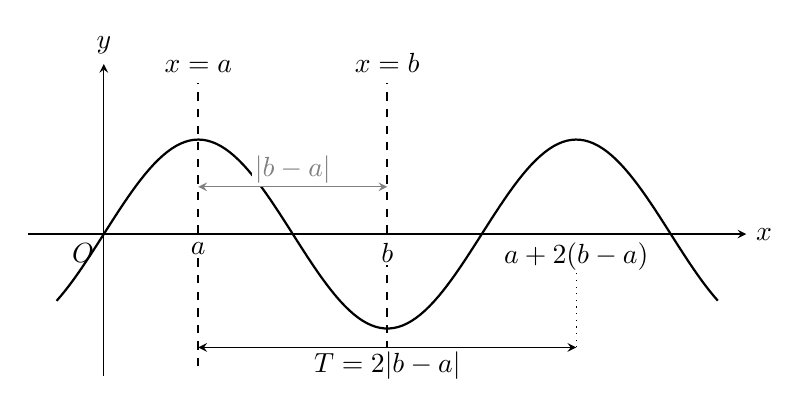
\begin{tikzpicture}[scale=1.2, >=stealth]
    % Axes
    \draw[->] (-0.8,0) -- (6.8,0) node[right] {$x$};
    \draw[->] (0,-1.5) -- (0,1.8) node[above] {$y$};
    \node[below left] at (0,0) {$O$};
    
    % Periodic function cos(pi/2 * (x-1))
    \draw[thick, domain=-0.5:6.5, samples=150] plot (\x, {cos(90*(\x-1))});
    
    % Symmetry axes
    \draw[dashed, thick] (1,-1.4) -- (1,1.6) node[above] {$x=a$};
    \draw[dashed, thick] (3,-1.4) -- (3,1.6) node[above] {$x=b$};
    
    % Axis labels
    \node[below, yshift=-2pt, fill=white, inner sep=1pt] at (1,0) {$a$};
    \node[below, yshift=-2pt, fill=white, inner sep=1pt] at (3,0) {$b$};
    
    % Spacing indicators
    \draw[<->, gray, thin] (1,0.5) -- (3,0.5) node[midway, above, fill=white, inner sep=1pt] {$|b-a|$};
    \draw[<->, black, thin] (1,-1.2) -- (5,-1.2) node[midway, below, fill=white, inner sep=1.5pt] {$T = 2|b-a|$};
    \draw[dotted] (5, -1.2) -- (5,0);
    \node[below, yshift=-2pt, fill=white, inner sep=1pt] at (5,0) {$a+2(b-a)$};
  \end{tikzpicture}
  \par
  \small 双对称轴反射复合后的平移距离为 $2|b-a|$
\end{center}

\newpage

\begin{theorembox}{定理 2：双中心对称推周期}
  若函数 $f(x)$ 具有两个不同的对称中心 $(a, c)$ 和 $(b, c)$ ($a \neq b$，且纵坐标相同)，则 $f(x)$ 必为周期函数，且其一个周期为：
  \[ T = 2|b-a| \]
\end{theorembox}

\topicteachblock{代数推导}{
  根据关于 $(a, c)$ 和 $(b, c)$ 中心对称的定义，有：
  \[ f(x) + f(2a-x) = 2c \quad \text{且} \quad f(x) + f(2b-x) = 2c \]
  两式相减消去常数 $2c$，可得：
  \[ f(2a-x) = f(2b-x) \]
  令 $u = 2a-x$，则 $x = 2a-u$，代入右侧自变量得 $2b-x = 2b-(2a-u) = u + 2(b-a)$。\\
  从而有：
  \[ f(u) = f(u + 2(b-a)) \]
  故其一个周期为 $T = 2|b-a|$。
}

\topicteachblock{几何直观与图示}{
  在图像上，连续绕两个不同的对称中心（且高度相同）旋转 $180^\circ$，其复合效果消除了旋转的倾斜，等价于沿 $x$ 轴水平平移了 $2|b-a|$ 的距离。
}

\begin{center}
  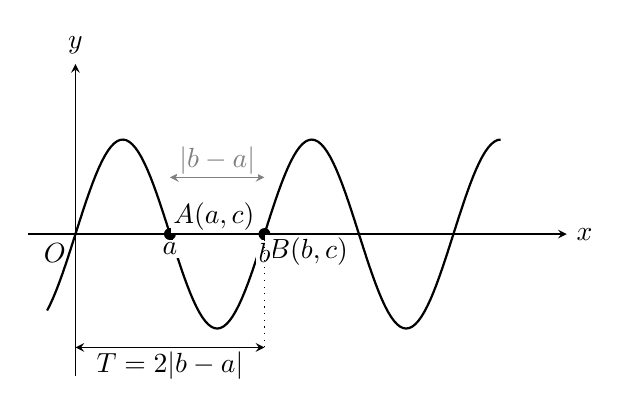
\begin{tikzpicture}[scale=1.2, >=stealth]
    % Axes
    \draw[->] (-0.5,0) -- (5.2,0) node[right] {$x$};
    \draw[->] (0,-1.5) -- (0,1.8) node[above] {$y$};
    \node[below left] at (0,0) {$O$};
    
    % Periodic function sin(pi * x)
    \draw[thick, domain=-0.3:4.5, samples=150] plot (\x, {sin(180*\x)});
    
    % Symmetry centers on x-axis
    \fill (1,0) circle (1.8pt) node[above right, fill=white, inner sep=1pt] {$A(a,c)$};
    \fill (2,0) circle (1.8pt) node[below right, fill=white, inner sep=1pt] {$B(b,c)$};
    
    \node[below, yshift=-2pt, fill=white, inner sep=1pt] at (1,0) {$a$};
    \node[below, yshift=-2pt, fill=white, inner sep=1pt] at (2,0) {$b$};
    
    % Spacing indicators
    \draw[<->, gray, thin] (1,0.6) -- (2,0.6) node[midway, above, fill=white, inner sep=1pt] {$|b-a|$};
    \draw[<->, black, thin] (0,-1.2) -- (2,-1.2) node[midway, below, fill=white, inner sep=1.5pt] {$T = 2|b-a|$};
    \draw[dotted] (0, -1.2) -- (0,0);
    \draw[dotted] (2, -1.2) -- (2,0);
  \end{tikzpicture}
  \par
  \small 两个同高对称中心连续绕行复合后的平移距离为 $2|b-a|$
\end{center}

\newpage

\begin{theorembox}{定理 3：一轴一中心对称推周期}
  若函数 $f(x)$ 图像关于直线 $x = a$ 轴对称，且关于点 $(b, c)$ 中心对称 ($a \neq b$)，则 $f(x)$ 必为周期函数，且其一个周期为：
  \[ T = 4|b-a| \]
\end{theorembox}

\topicteachblock{代数推导}{
  由关于直线 $x=a$ 轴对称得：$f(x) = f(2a-x)$。\\
  由关于点 $(b, c)$ 中心对称得：$f(x) + f(2b-x) = 2c \implies f(2b-x) = 2c - f(x)$。\\
  用 $2a-x$ 代替第二式中的 $x$，得：
  \[ f(2b-(2a-x)) = 2c - f(2a-x) \]
  代入第一式 $f(2a-x) = f(x)$，整理可得：
  \[ f(x + 2(b-a)) = 2c - f(x) \]
  这是典型的反周期（反相）关系。我们将自变量再次平移 $2(b-a)$ 距离，代入上式：
  \[ f(x + 4(b-a)) = 2c - f(x + 2(b-a)) = 2c - (2c - f(x)) = f(x) \]
  即 $f(x + 4(b-a)) = f(x)$，函数表现出周期性，一个周期为 $4|b-a|$。
}

\topicteachblock{几何直观与图示}{
  一次反射（折叠）和一次中心对称旋转的复合会导致函数值反相（即上凸部分变成下凹部分）。因此，平移 $2|b-a|$ 只能得到反相图像；只有连续进行两次上述复合操作（共四次对称变换），将反相图像再次翻转，才能完全复原，故周期为两对称元间距的 $4$ 倍。
}

\begin{center}
  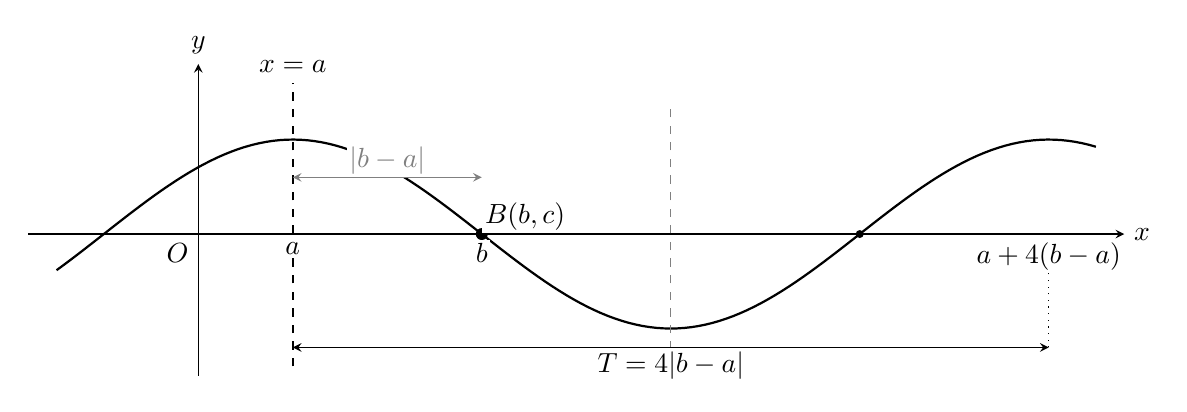
\begin{tikzpicture}[scale=1.2, >=stealth]
    % Axes
    \draw[->] (-1.8,0) -- (9.8,0) node[right] {$x$};
    \draw[->] (0,-1.5) -- (0,1.8) node[above] {$y$};
    \node[below left] at (0,0) {$O$};
    
    % Periodic function cos(45 * (x-1))
    \draw[thick, domain=-1.5:9.5, samples=150] plot (\x, {cos(45*(\x-1))});
    
    % Symmetry elements
    \draw[dashed, thick] (1,-1.4) -- (1,1.6) node[above] {$x=a$};
    \fill (3,0) circle (1.8pt) node[above right, fill=white, inner sep=1pt] {$B(b,c)$};
    
    \node[below, yshift=-2pt, fill=white, inner sep=1pt] at (1,0) {$a$};
    \node[below, yshift=-2pt, fill=white, inner sep=1pt] at (3,0) {$b$};
    
    % Next elements for period visualization
    \draw[dashed, gray] (5,-1.4) -- (5,1.4);
    \fill (7,0) circle (1.2pt);
    
    % Spacing indicators
    \draw[<->, gray, thin] (1,0.6) -- (3,0.6) node[midway, above, fill=white, inner sep=1pt] {$|b-a|$};
    \draw[<->, black, thin] (1,-1.2) -- (9,-1.2) node[midway, below, fill=white, inner sep=1.5pt] {$T = 4|b-a|$};
    \draw[dotted] (9, -1.2) -- (9,0);
    \node[below, yshift=-2pt, fill=white, inner sep=1pt] at (9,0) {$a+4(b-a)$};
  \end{tikzpicture}
  \par
  \small 一轴一中心反射绕行复合两次为反周期，复合四次为正周期 $4|b-a|$
\end{center}

\newpage

\section{板块五：典型真题精讲与板书规范}

\teachquestionheader{抽象函数周期与对称综合推导}
\teachvalue{本题考查学生在考场上遇到抽象函数关系式时的推导逻辑，重点考查定义域、周期性、对称性的代数转换以及特定函数值的求解。}

\begin{exbox}{典型真题}
  已知定义在 $\mathbb{R}$ 上的奇函数 $f(x)$ 满足 $f(x+2) = -f(x)$，且当 $x \in (0, 1]$ 时，$f(x) = 2^x - 1$。
  \begin{enumerate}
    \item 求 $f(x)$ 的周期；
    \item 证明 $f(x)$ 关于直线 $x = 1$ 对称；
    \item 求 $f(5.5)$ 的值。
  \end{enumerate}
\end{exbox}

\begin{paracol}{2}
\topicteachblock{标准解答与板书规范}{
  解：(1) 因为对任意 $x \in \mathbb{R}$，都有 $f(x+2) = -f(x)$，\\
  所以 $f(x+4) = f((x+2)+2) = -f(x+2) = -(-f(x)) = f(x)$，\\
  故 $f(x)$ 是周期函数，且其一个周期为 $T = 4$。\\
  \vspace{0.4em}
  (2) 证明：因为 $f(x)$ 是定义在 $\mathbb{R}$ 上的奇函数，\\
  所以对任意 $x \in \mathbb{R}$，有 $f(-x) = -f(x)$。\\
  又因为 $f(x+2) = -f(x)$，以 $-x$ 代替 $x$ 得：
  \[ f(2-x) = -f(-x) \]
  将奇函数关系式 $f(-x) = -f(x)$ 代入，得：
  \[ f(2-x) = -(-f(x)) = f(x) \]
  即 $f(1+(1-x)) = f(1-(1-x))$，\\
  由对称性定义可知，函数 $f(x)$ 的图像关于直线 $x = 1$ 对称。\\
  \vspace{0.4em}
  (3) 利用周期性，有：
  \[ f(5.5) = f(5.5 - 4) = f(1.5) \]
  利用关于 $x = 1$ 的轴对称性，有：
  \[ f(1.5) = f(2 - 1.5) = f(0.5) \]
  因为 $0.5 \in (0, 1]$，代入解析式得：
  \[ f(0.5) = 2^{0.5} - 1 = \sqrt{2} - 1 \]
  所以 $f(5.5) = \sqrt{2} - 1$。
}

\switchcolumn
\topicteachblock{学生问题诊断与思维防线}{
  \errortag{周期与对称条件混淆}
  学生容易写成 $f(1.5) = -f(-0.5)$ 或其他错误替换，在周期变换与对称变换中发生错乱。\\
  \textbf{课堂纠偏策略}：
  要求学生在草稿纸上把计算过程写成“链式变形”，每一步都要明确写出依据。例如：
  \[ f(5.5) \xrightarrow{\text{依据：周期 } T=4} f(1.5) \xrightarrow{\text{依据：对称轴 } x=1} f(0.5) \]
  这种“链式变形书写规范”能有效防止学生在中途发生符号和公式的代数错乱。
  \vspace{0.6em}
  \remedy{
    若学生无法独立完成第二问关于 $x=1$ 对称的代数证明，课后必须默写“对称轴 $x=a$ 对应的两个等价代数式”；若在求 $f(5.5)$ 时带入错误区间，需重做本专题后面关于抽象函数求值的不等式变式。
  }
}
\end{paracol}

\newpage

\section{教师建议与记忆口诀卡片}

\begin{warnbox}{终极记忆口诀（建议要求学生大声朗读并抄写）}
  \large
  \[ \text{单调看增减，奇偶看正负；} \]
  \[ \text{轴对左右等，中心左右和；} \]
  \[ \text{两轴推双倍，两点亦同理；} \]
  \[ \text{一轴一中心，四倍得周期。} \]
\end{warnbox}

\begin{teachbox}{教学反思与重难点落实口诀解释}
  \begin{enumerate}
    \item \textbf{轴对左右等}：$f(a+x) = f(a-x)$。自变量偏离对称轴 $a$ 的左右两侧，其函数值是相等的。
    \item \textbf{中心左右和}：$f(a+x) + f(a-x) = 2b$。自变量偏离中心横坐标 $a$ 的左右两侧，其函数值相加是一个固定的常数 $2b$。
    \item \textbf{两轴推双倍}：对称轴 $x=a$ 与 $x=b$ 叠加，周期是间距的两倍，$T = 2|b-a|$。
    \item \textbf{两点亦同理}：对称中心 $(a, c)$ 与 $(b, c)$ 叠加，周期是间距的两倍，$T = 2|b-a|$。
    \item \textbf{一轴一中心，四倍得周期}：对称轴 $x=a$ 与对称中心 $(b, c)$ 叠加，周期是间距的四倍，$T = 4|b-a|$。
  \end{enumerate}
\end{teachbox}

\end{document}
